\subsection*{Problema 24}

\textbf{Enunciado:}
Calcular la integral indefinida:
\begin{align*}
\int \frac{dx}{x \sqrt{x^2 + 1}}
\end{align*}

\textbf{Solución:}
Para resolver esta integral, utilizaremos el método de sustitución trigonométrica. 

Definimos la sustitución:
\begin{align*}
x &= \tan\theta \\
dx &= \sec^2\theta \, d\theta
\end{align*}

Además, el término radical se simplifica como:
\begin{align*}
\sqrt{x^2 + 1} &= \sqrt{\tan^2\theta + 1} \\
&= \sqrt{\sec^2\theta} = \sec\theta
\end{align*}

Sustituimos $x$, $dx$ y el radical en la integral original:
\begin{align*}
\int \frac{\sec^2\theta \, d\theta}{\tan\theta \cdot \sec\theta}
\end{align*}

Simplificamos la expresión trigonométrica:
\begin{align*}
&= \int \frac{\sec\theta}{\tan\theta} \, d\theta \\
&= \int \left(\frac{1}{\cos\theta}\right) \left(\frac{\cos\theta}{\sin\theta}\right) d\theta \\
&= \int \csc\theta \, d\theta
\end{align*}

La integral de la cosecante es conocida:
\begin{align*}
&= \ln \left| \csc\theta - \cot\theta \right| + C
\end{align*}

A partir del triángulo rectángulo asociado a $\tan\theta = x$, tenemos que la hipotenusa es $\sqrt{x^2+1}$, por lo que:
\begin{align*}
\csc\theta &= \frac{\sqrt{x^2 + 1}}{x} \\
\cot\theta &= \frac{1}{x}
\end{align*}

Sustituimos estos valores en la solución:
\begin{align*}
&= \ln \left| \frac{\sqrt{x^2+1}}{x} - \frac{1}{x} \right| + C \\
&= \ln \left| \frac{\sqrt{x^2+1} - 1}{x} \right| + C
\end{align*}

\textbf{Resultado Final:}
\begin{align*}
\int \frac{dx}{x \sqrt{x^2 + 1}} = \ln \left| \frac{\sqrt{x^2+1} - 1}{x} \right| + C
\end{align*}

\begin{figure}[H]
	\centering
	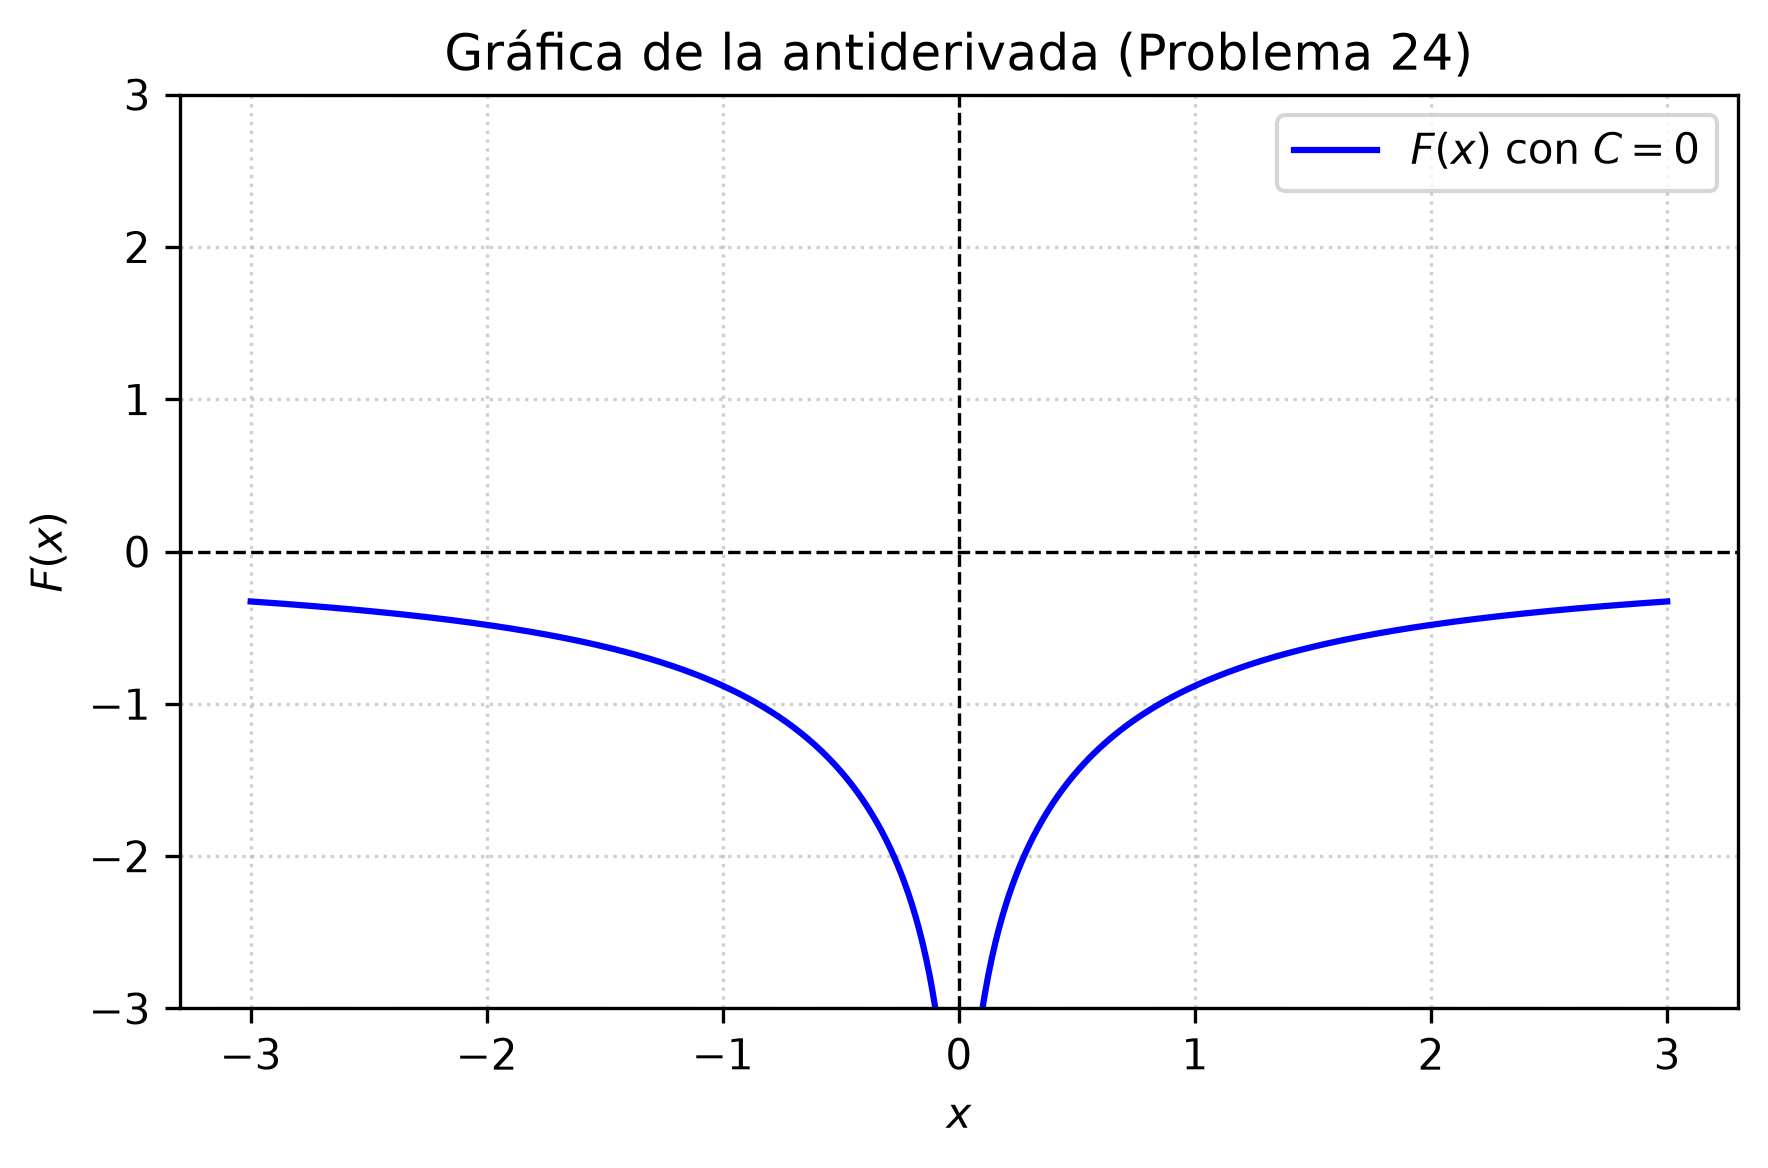
\includegraphics[width=\columnwidth]{semana_05/graficas/SEM05_P24_grafica.png}
	\caption{Representación gráfica de $f(x)$ y su antiderivada $F(x)$ evaluada para la constante de integración $C = 0$ (Problema 24).}
	\label{fig:problema24}
\end{figure}
